\documentclass{optica-article}
\usepackage{xcolor} 
\definecolor{darkred}{HTML}{BA1A1A}
\definecolor{extralightgray}{HTML}{F5F5F5}

\journal{opticajournal} % for journals or Optica Open

\articletype{Research Article}

\usepackage{lineno}
\usepackage{todonotes}
\usepackage{xcolor}
\usepackage{soul}
\providecommand{\tightlist}{%
  \setlength{\itemsep}{0pt}\setlength{\parskip}{0pt}}
\linenumbers % Turn off line numbering for Optica Open preprint submissions.

\begin{document}

\title{Data Recovery and Pulse Position Modulation with a Photon Number Resolving SNSPD}

\author{Andrew Mueller\authormark{1, 2, *}, Boris Korzh\authormark{2}, Emma Wollman\authormark{2}, Andrew D. Beyer\authormark{2}, Matthew D. Shaw\authormark{2}, and Maria Spiropulu\authormark{3}}

\address{\authormark{1}Applied Physics, California Institute of Technology, 1200 E California Blvd., Pasadena, CA, 91125, USA \\
\authormark{2}Jet Propulsion Laboratory, California Institute of Technology, 4800 Oak Grove Dr., Pasadena, CA, 91109, USA \\
\authormark{3}Division of Physics, Mathematics and Astronomy, California Institute of Technology, 1200 E California Blvd., Pasadena, CA 91125, USA }

\email{\authormark{*}andrewstermueller@gmail.com} %% email address is required; see note below about the corresponding author designation

% use {asbstract*} to suppress the copyright line. Copyright information will be added in production

\begin{abstract*} 
Superconducting Nanowire Single Photon Detectors have leading low-jitter performance, especially in the mid-infrared. They are useful for classical communication over high loss channels --such as across deep space-- and for quantum communication for which signals are restricted to the few-photon level. For classical communication, high photon information efficiency communication may be achieved with Pulse Position Modulation (PPM) whereby data is encoded in the arrival time of an optical pulse with respect to a clock. In the process of demonstrating PPM on a 20~Ghz clock, we study the effects of Photon Number Resolution (PNR) in new low-jitter types of SNSPDs. These PNR effects complicate fixed-threshold triggering of RF pulses from the SNSPD, and corrupt arrival time measurements if not properly managed. We demonstrate methods for simultaneous arrival time and photon number measurement which enables high clock rate PPM for space applications as well as high rate quantum communication and computing applications that benefit from photon number resolution.
\end{abstract*}

%%%%%%%%%%%%%%%%%%%%%%%%%%  body  %%%%%%%%%%%%%%%%%%%%%%%%%%
\hypertarget{introduction}{%
\section{Introduction}\label{introduction}}

Deep space optical communication has been a growing field of study in recent years, as space agencies look for ways to increase data rates to and from deep space missions. A key challenge in this work is closing a communication link over extremely large distances and high loss. For data transmission from a power-limited spacecraft to earth, this must be done with a restricted power budge, and therefore requires the use of photon efficient communication protocols that optimize the number of bits sent per unit of energy.

In this article, we demonstrate high rate Pulse Position Modulation (PPM) applicable to future deep space communication. A transmitter sends an optical pulse in one of $2^M$ possible time slots measured with respect to a clock. At a receiver, the arrival time of this pulse is measured to recover $M$ bits of encoded data. Each successive set of $2^M$ time slots following by a dead time constitute a PPM frame.

The Deep Space Optical Communicaiton (DSOC) project managed by the Jet Propulsion Laboratory (JPL) demonstrates optical communication using PPM with the Psyche spacecraft from distances of 0.06 to 2.7 Au \cite{Srinivasan2023GroundReceiver}.

For larger M, more data may be sent with a single optical pulse or given spacecraft power budge. This is quantified through the photon information efficiency $c_p = C/E$ where $C$ is the link capacity

$$
C=\left(1-e^{-E}\right) \log _2 M,
$$

and $E$ is the photon cost per optical pulse. DSOC relies on modulation of a CW seed laser to generate the communication signal on the spacecraft. This signal is then amplified by an Erbium Doped Fiber Amplifier (EDFA) which dominates the power budget of the spacecraft optical transmission system. Therefore, power consumption scales with the number of optical pulses sent.

The DSOC project uses PPM with maximum M values of at least 5, meaning 5 bits of data are sent using 32 time slots per frame. M values as high as 19 have been demonstrated in the lab~\cite{essiambre2023record}, but the number of time bins needed per frame scales exponentially with the number of bits transmitted per pulse. Therefore, for a given fixed clock rate and time bin duration, the PPM data rate decreases dramatically for higher M values.

We demonstrate a high clock rate PPM protocol in the lab based on modulating a mode-locked laser and receiving pulses with a low jitter superconducting nanowire single photon detector (SNSPD) (fig.~\ref{fig:intro} (a)). We focus on demonstrating moderately high PIE, while also increasing the clock rate of the sytem by an order of magnitude relative to the DSOC platform (from 2~GHz to 20~GHz). By operating at both higher clock rate and PIE than DSOC, this system exemplifies how future iterations of DSOC may send data more quickly but also over greater distances with the same power budget.

The rate increase is possible due to recent advancements in Niobium Nitride SNSPDs~\cite{Colangelo2023}. These achieve low jitter performance by incorporating impedance matching tapers for efficient RF coupling, resulting in higher slew rate pulses, and by enabling RF pulse readout from both ends of the nanowire. The dual-ended readout allows for the cancellation of jitter caused by the variable location of photon arrival along the meander when the differential signals are recombined with a balun. These detectors achieve jitter as low as 50 ps at the FW(1/100)M level, making them suitable for the demonstration of PPM with 50 ps slot widths and a 20 GHz clock.

\hypertarget{fig:intro}{%
\begin{figure}
\centering
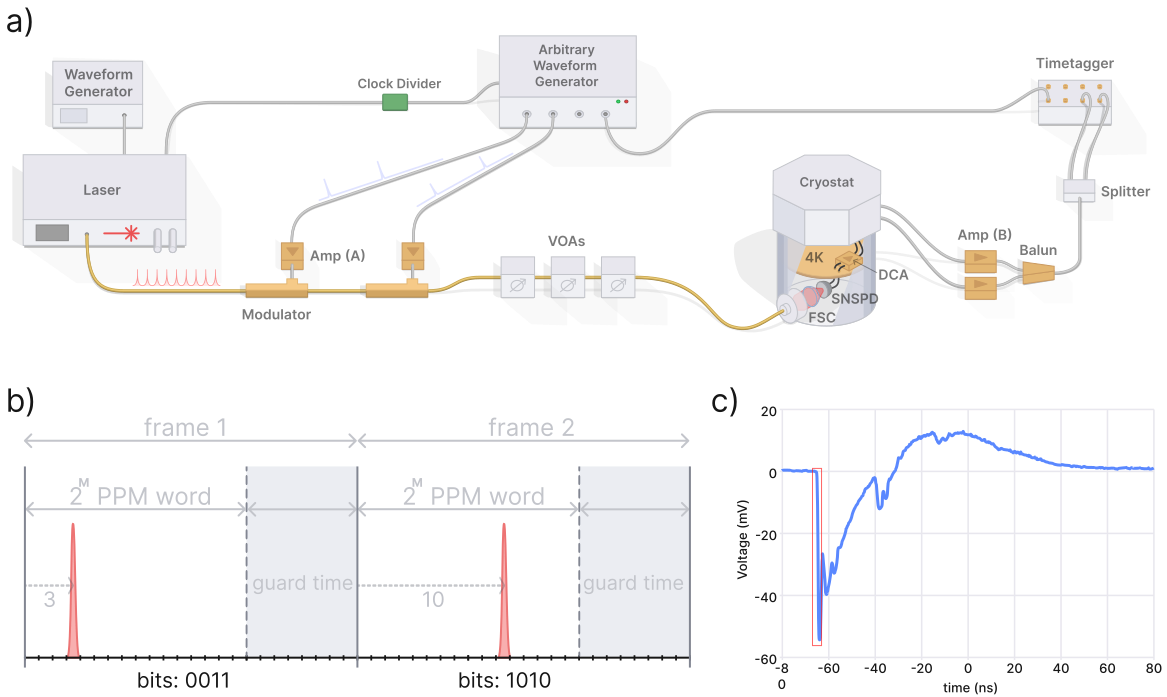
\includegraphics[width=1\textwidth]{./figs/fig_intro_2_light.pdf}
\caption[{PPM modulation and experiment setup}]{\textbf{PPM modulation and experiment setup} a) Diagram of the expiremental setup. WG: wave generator, CD: clock divider board, AWG: Arbitrary Waveform Generator, MLL: Mode Locked Laser (Pritel UAC), IM: Intensity Modulator, BC: Bias Controller, FSC: Free Space Coupling System, DCA: DC Coupled Cryo-amp b) How bits are transmitted in M=16 PPM modulation. An optical pulse is transmitted with a clock-referenced integer delay which encodes 4 bits of data. c) Scope trace of the RF pulse produced by the differential-readout tapered SNSPD. fig.~\ref{fig:waveform} zooms in on the rising edge outlined in red here.}
\label{fig:intro}
\end{figure}
}

However, these detectors exhibit a photon number dependent response that affects the time-correlated measurements needed for high-rate PPM. This behavior, shown in Fig.~\ref{fig:waveform} also gives the detector photon number resolution (PNR) --- a property that is desirable in certain applications including quantum communication and quantum computing. The SNSPD generates RF pulses with greater amplitude and slew rate when detecting optical pulses with multiple photons. Photon number effects are especially evident in this lower jitter variety of SNSPD due to the use of impedance matching tapers which more efficiently couple energy out of the nanowire and into the readout circuit. With high resolution time tagging equipment, photon number dependent effects have even been observed in SNSPDs not necessarily designed to exhibit it \cite{schapeler2023superconducting, sauer2023resolving} like those without tapers \cite{Cahall2017SlewRatePNR}. Therefore it is increasingly likely that future research involving low-jitter SNSPDs and multiphoton pulsed sources will have to explicitly manage the PNR response for accurate time-correlated measurements -- whether the effect it is desired or not.

For the tapered differential detectors, the PNR response affects timing of fixed threshold timetaggs at any trigger level (fig.~\ref{fig:waveform}). However, at lower trigger levels the PNR response is less pronounced and the timing measurements are less affected. Therefore, we divide a single SNSPD readout line using an RF splitter and trigger on the RF pulse at a high and low level as shown by the red lines in fig.~\ref{fig:waveform}. This gives partially conjugate information on optical pulse arrival time and photon number. From these measurements we study the PNR response in detail and present two methods for managing it. We demonstrate how the photon number information may be deconvolved from the arrival time information, and how both de-correlated degrees of freedom can be extracted simultaneously. This enables the original goal of high rate PPM, but also informs how low-jitter photon number resolving SNSPDs can be used in other classical communication and quantum applications.

\hypertarget{fig:waveform}{%
\begin{figure}
\centering
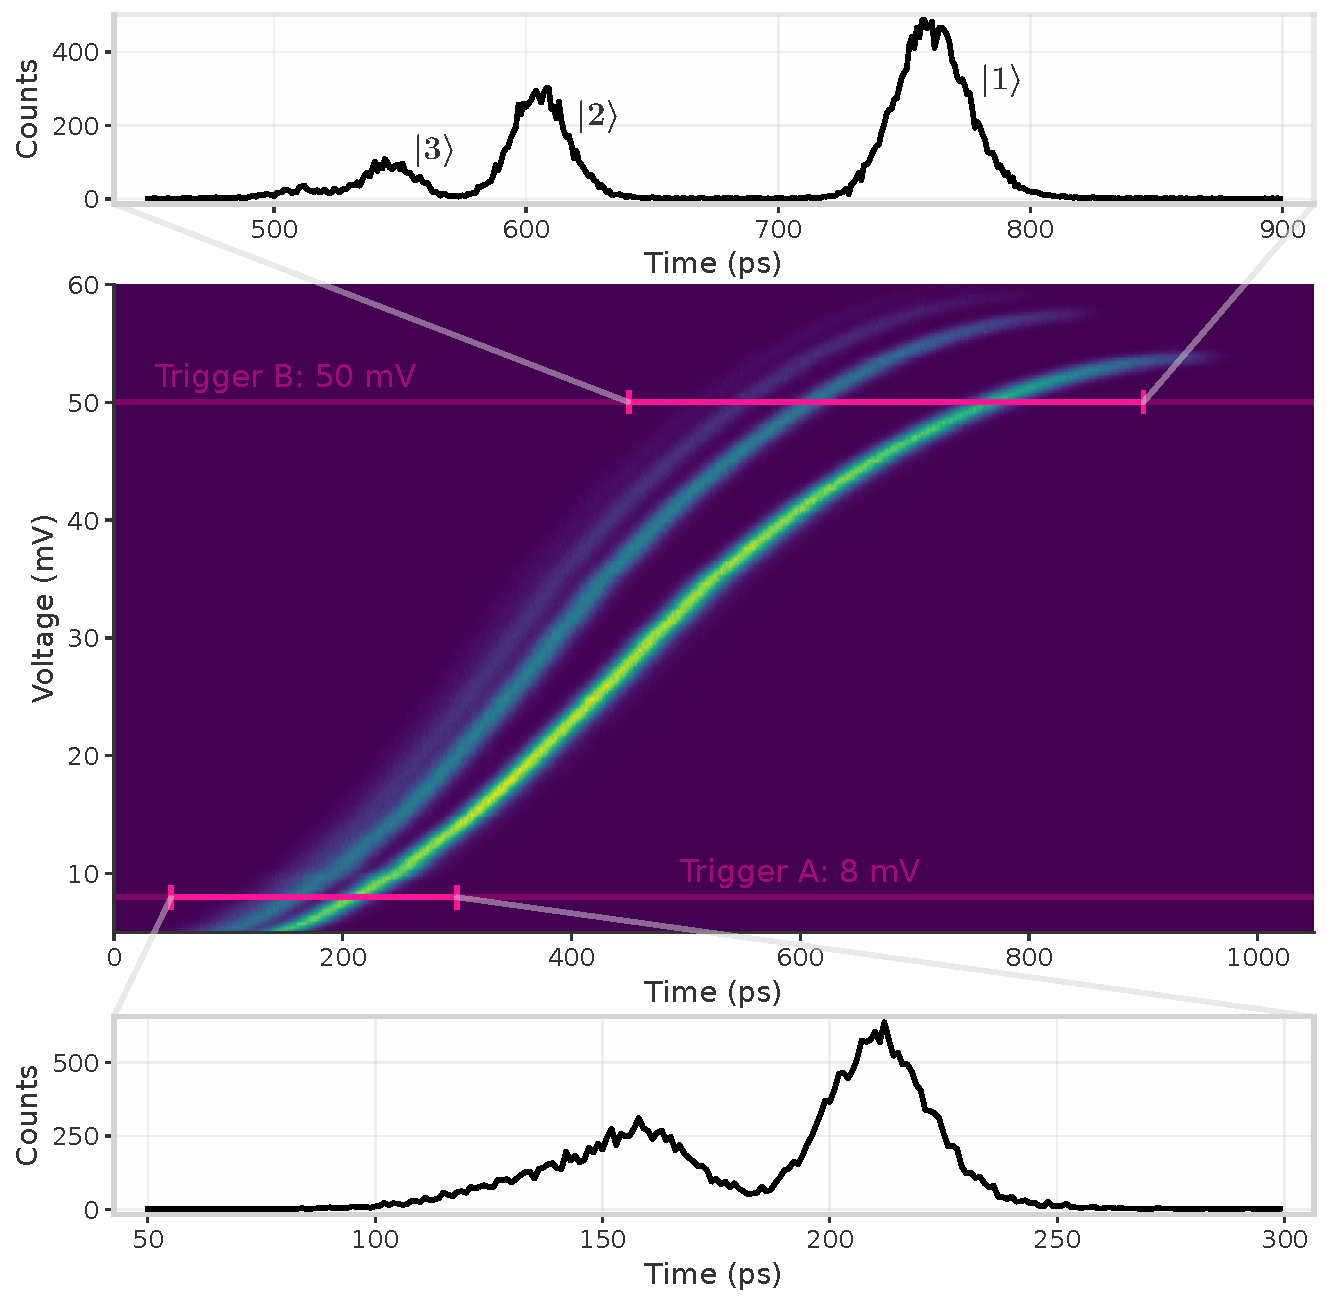
\includegraphics[width=0.8\textwidth]{./figs/waveform_light.pdf}
\caption[{PNR-sensitive pulse waveform}]{\textbf{PNR-sensitive pulse waveform} The rising edge of the differential SNSPD's RF pulses exhibit variations in height, slew rate, and arrival time due to photon-number dependent dynamics. The slopes of the 1-photon and 2-photon pulses significantly differ, and as the photon number increases, the alterations to the pulse shape become progressively smaller. Trigger levels A (8~mV) and B (50~mV) were used to extract as much information about pulse slope and arrival time as possible.}
\label{fig:waveform}
\end{figure}
}

\hypertarget{development-of-a-modulation-source}{%
\subsection{Development of a modulation source}\label{development-of-a-modulation-source}}

We produce our PPM signal signal by carving a 1550~nm high rate mode locked laser with lithium niobate modulators. Each mode locked laser pulse has duration on the order of 0.5~ps. By modulating a mode-locked laser,
the optical pulses do not incur timing jitter from the limited slew rate of the modulators or the RF signal that drives them. Two modulators are used in series to achieve the high extinction ratio needed to successively block up to 2047 laser pulses in a row.

We do two PPM demonstrations, with the source mode locked laser operating at 10.75 and 20 GHz. THe 10.75 GHz demonstration uses a M value of 10, thereby making frames with 1024 time slots of 93 ps width each. The 20 GHz demonstration uses M=11, giving 2048 time slots per frame of 50 ps width. Each frame ends with a dead time of approximately 150 ns to allow the SNSPD to fully recover before the next frame.

Several modern free running time taggers support the averaging of multiple input channels to create fewer higher resolution channels. This implies a tradeoff between jitter or timing resolution and number of channels for a given time tagging device. Therefore, it is important to consider readout methods like that presented here that make use of 2 lower-resolution channels in place of a single higher resolution channel, as these two configurations are similarly resource efficient.

\hypertarget{methods}{%
\section{Methods}\label{methods}}

We encode a 98 kilobit image (fig.~\ref{fig:decoding_20GHz} b) as the dataset for transmission in both the 10.75 and 20 Ghz demonstrations. Due to limitations of the AWG, the full dataset can not be transmitted sequentially. Instead, sequencies of 8 (10.75 Ghz) and 9 (20 GHz) pulses each are successively loaded into AWG memory, transmitted several times, then switched out for the next sequence. The 98 kbit dataset is therefore transmitted with 9832 (10.75 GHz) and 8937 (20 GHz) frames across 1229 (10.75 GHz) and 993 (20 GHz) AWG sequences. Assuming sequential transmission of all frames, the 10~GHz demonstration achieves a data rate of 40.7 megabits/s, and the 20~GHz demonstration achieves 43.6 megabits/s.

We begin with a preamble sequence that only consists of pulses in the $i = 0$ time slot. Before sending the rest of the dataset, we modulate this set multiple times, collecting data from low and high trigger levels for impinging optical pulses of varying mean photon number. This provides information on the detector's photon number response without arrival time variation. We label the measurements from the low (8~mV) and high (50~mV) trigger levels as $t_A$ and $t_B$, respectively. As shown in Fig.~\ref{fig:waveform}, histograms of these arrival events are multimodal with distinct groupings for for each photon number detection. We first present a method for recovering a symmetric arrival time response function using the the slope measurement $\Delta t_{BA} = t_B - t_A$.

\hypertarget{slope-based-correction}{%
\subsection{Slope-based correction}\label{slope-based-correction}}

\hypertarget{fig:slope_correction}{%
\begin{figure}
\centering
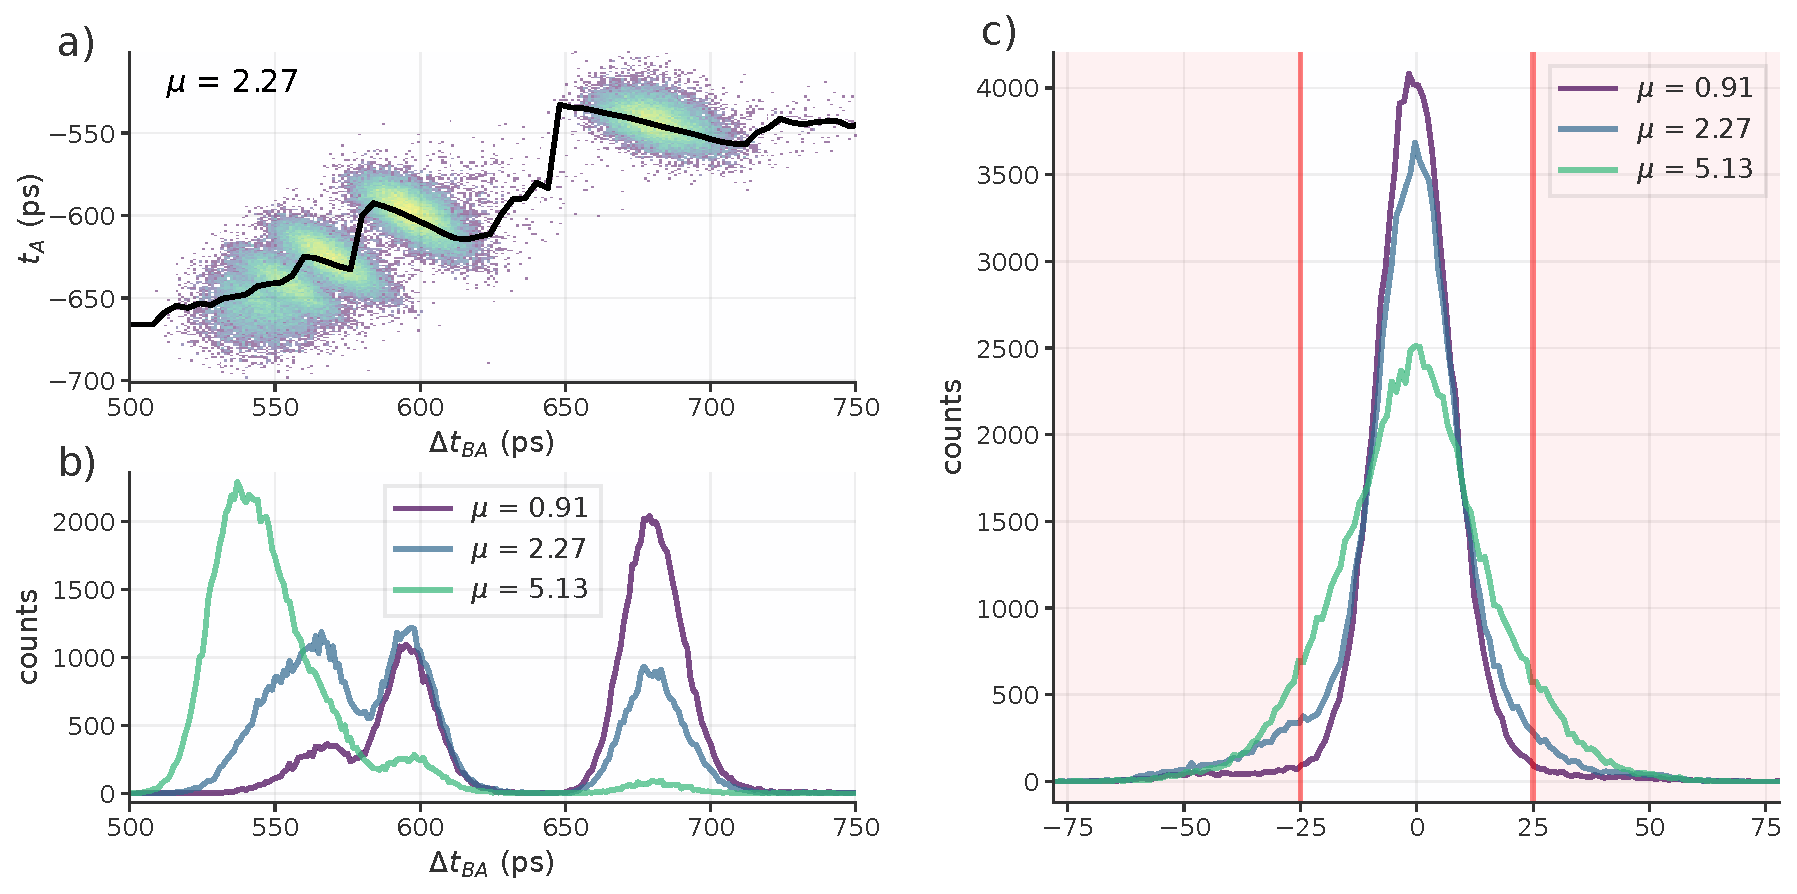
\includegraphics[width=1\textwidth]{./figs/slope_cancellation_light.pdf}
\caption[{PNR slope variation analysis and cancellation}]{\textbf{PNR slope variation analysis and cancellation} a) 2D histogram of RF pulse measurements. Through graphing slope $\Delta t_{BA}$ on the x-axis and arrival time $t_A$ on the y-axis, a series of groupings are visible that identify the discrete photon numbers detected. b) Histogram of events for pulse slope $\Delta t_{BA}$ for several mean photon numbers. c) Histogram of constructed measurements $\tilde{t_A}$ from applying pulse-slope-dependent corrections $C_A$. The distribution of $\tilde{t_A}$ is symmetric, but its FWHM width varies depending on mean photon number.}
\label{fig:slope_correction}
\end{figure}
}

Pairs of pulse measurements $t_A$ and $t_B$ may be graphed on a 2D plane parametrized by $\Delta t_{BA}$ on the x-axis and $t_A$. fig.~\ref{fig:slope_correction} a shows how this protection exhibits multiple groupings that correspond the the photon number character of the impinging optical mode. The 1 and 2-photon events are clearly identifiable and seperated from other events, with $|3\rangle$, $|4\rangle$, and $|5\rangle$ events also visible with less mutual separation. While fig.~\ref{fig:slope_correction} a is shown here for just one mean photon number $\mu$, this response is collected for a full range of attenuations and corresponding $\mu$. fig.~\ref{fig:slope_correction} a shows histograms from projecting 3 such measurements down onto the $\Delta t_{BA}$ axis.

The slope-correction method involves the measurement and creation of a slope-versus-arrival time line, one of which is shown in black on fig.~\ref{fig:slope_correction} a. This is produced by averaging all $t_A$ measurements for a given slope $\Delta t_{BA}$, or equivalently averaging across rows for each column in the 2D plotted data in fig.~\ref{fig:slope_correction} a . By interpolating new $\Delta t_{BA}$ measurements on this curve and using it like a lookup table, PNR corrections $C_A$ are found. These may be subtracted off from $t_A$ producing $\tilde{t_A} = t_A - C_A(\Delta t_{BA})$ where $\tilde{t_A}$ is a constructed timing measurement that exhibits a symmetric arrival time response function and shown in fig.~\ref{fig:slope_correction} c.~

The data representation and calibration curve shown in fig.~\ref{fig:slope_correction} a may be constructed with $t_B$ on the y-axis as well. Then the PNR corrections are applied the the $t_B$ measurements instead. However, the resulting histograms $\tilde{t_B}$ are virtually identical to $\tilde{t_A}$ as they are ultimately constructed from the same data.

\hypertarget{cluster-analysis}{%
\subsection{Cluster analysis}\label{cluster-analysis}}

The photon-number dependent effects shown in Fig.~\ref{fig:waveform} are uniquely separable in terms of photon number due to the inherently pulsed nature of the source.

Given the pulsed nature of the modulation source, there is not necessarily a need to define a continuous variable like $\tilde{t_A}$ as an intermediate step before binning. Instead, PPM decoding can be generalized to the operation of matching a pair of timing measurements $t_A, t_B$ to one of multiple probability distributions in the $t_A, t_B$ space, each of which corresponds to a different time bin and models the photon number dynamics for that bin. The shape of the distributions is dependent on the mean photon number $\mu$, and they may overlap for shorter time bin lengths.

We opt to use a Gaussian mixture model (GMM) to model the detector response for a given time bin. This is a statistical model that represents the probability distribution of a set of data as a weighted sum of Gaussian distributions. It is effective for modelling the multi-model shape of the photon number dependent detector response with a minimal number of parameters. The ellipses in fig.~\ref{fig:gmm_model} a \& b represent Gaussians used to fit the histogrammed data. We use an off-the-shelf GMM algorithm, and do not impose any limit on how many Gaussians are used to faithfully model each one of the photon clusters.

\hypertarget{fig:gmm_model}{%
\begin{figure}
\centering
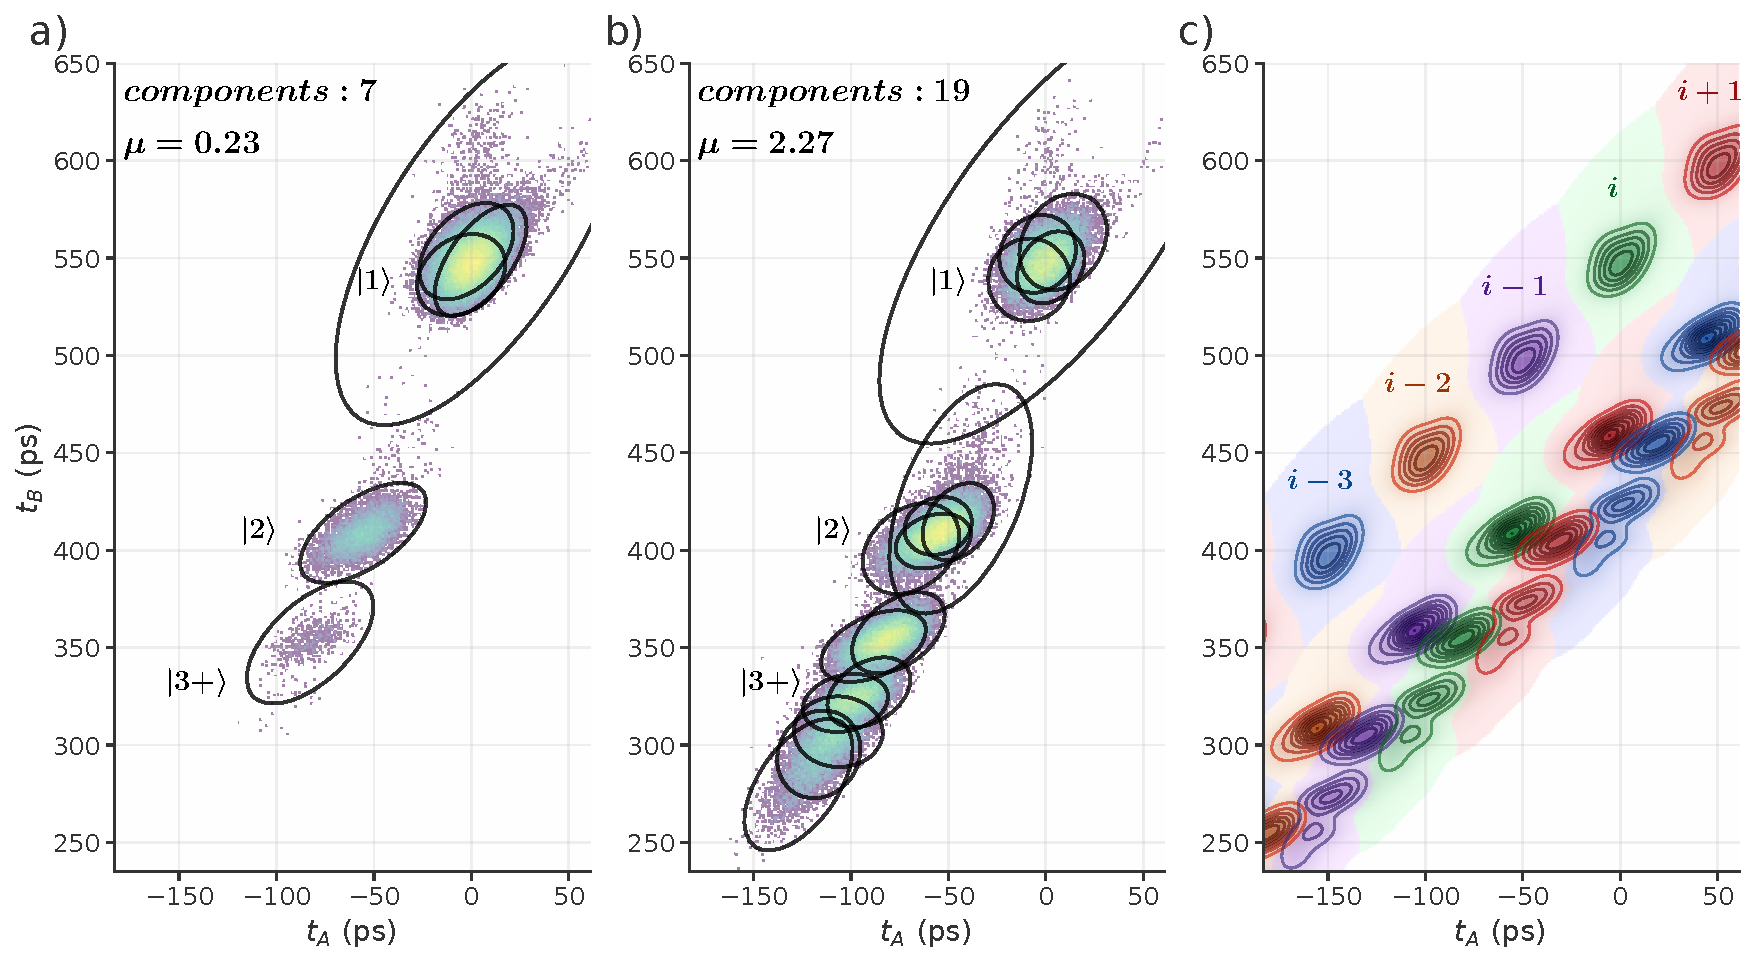
\includegraphics[width=1\textwidth]{./figs/gmm_intro_analysis_t_light.pdf}
\caption[{Initial Gaussian mixture model analysis}]{\textbf{Initial Gaussian mixture model analysis} a) \& b) 2D histogram of multi-photon SNSPD detections parametrized by timing measurements $t_A$ and $t_B$. The shape of the data and modelled distributions depends on mean photon number $\mu$. The ellipses denote the location and shape of the Gaussian components used to model the data. c) Shaded regions and overlayed contour plots for GMM-modeled detector response seperated by 50~ps, corresponding to the 20~GHz PPM demonstration. Identifying which bin a detector measurement corresponds to is equivalent to identifying which colored region a $t_A, t_B$ point should belong to. For the 20~GHz demonstration, discrimination cannot be perfect because the distributions overlap.}
\label{fig:gmm_model}
\end{figure}
}

Previous work has used principle component analysis (PCA) for modelling the photon-number dependent response of SNSPDs. As shown in section \ref{independent-component-analysis}, Independent Component Analysis (ICA) --- a method related to PCA --- is still useful for photon-number attribution for our detector and setup, and could be used in concert withe the slope-correction method above. However, as described in more detail in the discussion section, we believe the generality of the GMM approach has certain benefits, especially for future extensions to the analysis that must contend with pulse distortion effects like pile-up and time-walk~\cite{Mueller2023}. Ultimately, both GMM methods and PCA/ICA analysis methods hold promise for SNSPD further response modelling.

As shown in fig.~\ref{fig:gmm_model} c, there exist regions in the $t_A, t_B$ plane for which a given GMM model for pulse $i$ is most probable. The exact shape of this boundary could be computed as detailed in section \ref{computing-gmm-intersection-boundaries} for computationally efficient binning in the $t_A, t_B$ plane. But for this demonstration computational overhead this is not a major concern, so we compute the probability of a $[t_A, t_B]$ point for a few nearest distributions and pick the one with largest probability.

\hypertarget{results}{%
\section{Results}\label{results}}

For the full PPM decoding of both the 10~GHz and 20~GHz datasets, the constructed timetagg $\tilde{t_A}$ is first used to find an initial estimate for the correct time bin for each PPM frame. Then, the GMM analysis is performed for nearby time bins to create a correction to the initial estimate. For each of the 17 mean photon numbers for which we test PPM decoding, the GMM model is derived from fitting to the measurements from the preamble sequence of pulses in the i=0 time slot. fig.~\ref{fig:decoding_20GHz} a shows the decoding success and error rate for the 20~GHz demonstration, and
fig.~\ref{fig:decoding_20GHz} b shows the decoded image at 3 particular mean photon numbers indicated in fig.~\ref{fig:decoding_20GHz} a. As shown fig.~\ref{fig:decoding_20GHz} b and c, the photon number groupings of different time bins somewhat interleave with each other. Error rates with the GMM correction are therefore moderately lower, as it has better knowledge of the complex shape of the decision boundary between photon clusters in different time bins.

\hypertarget{fig:decoding_20GHz}{%
\begin{figure}
\centering
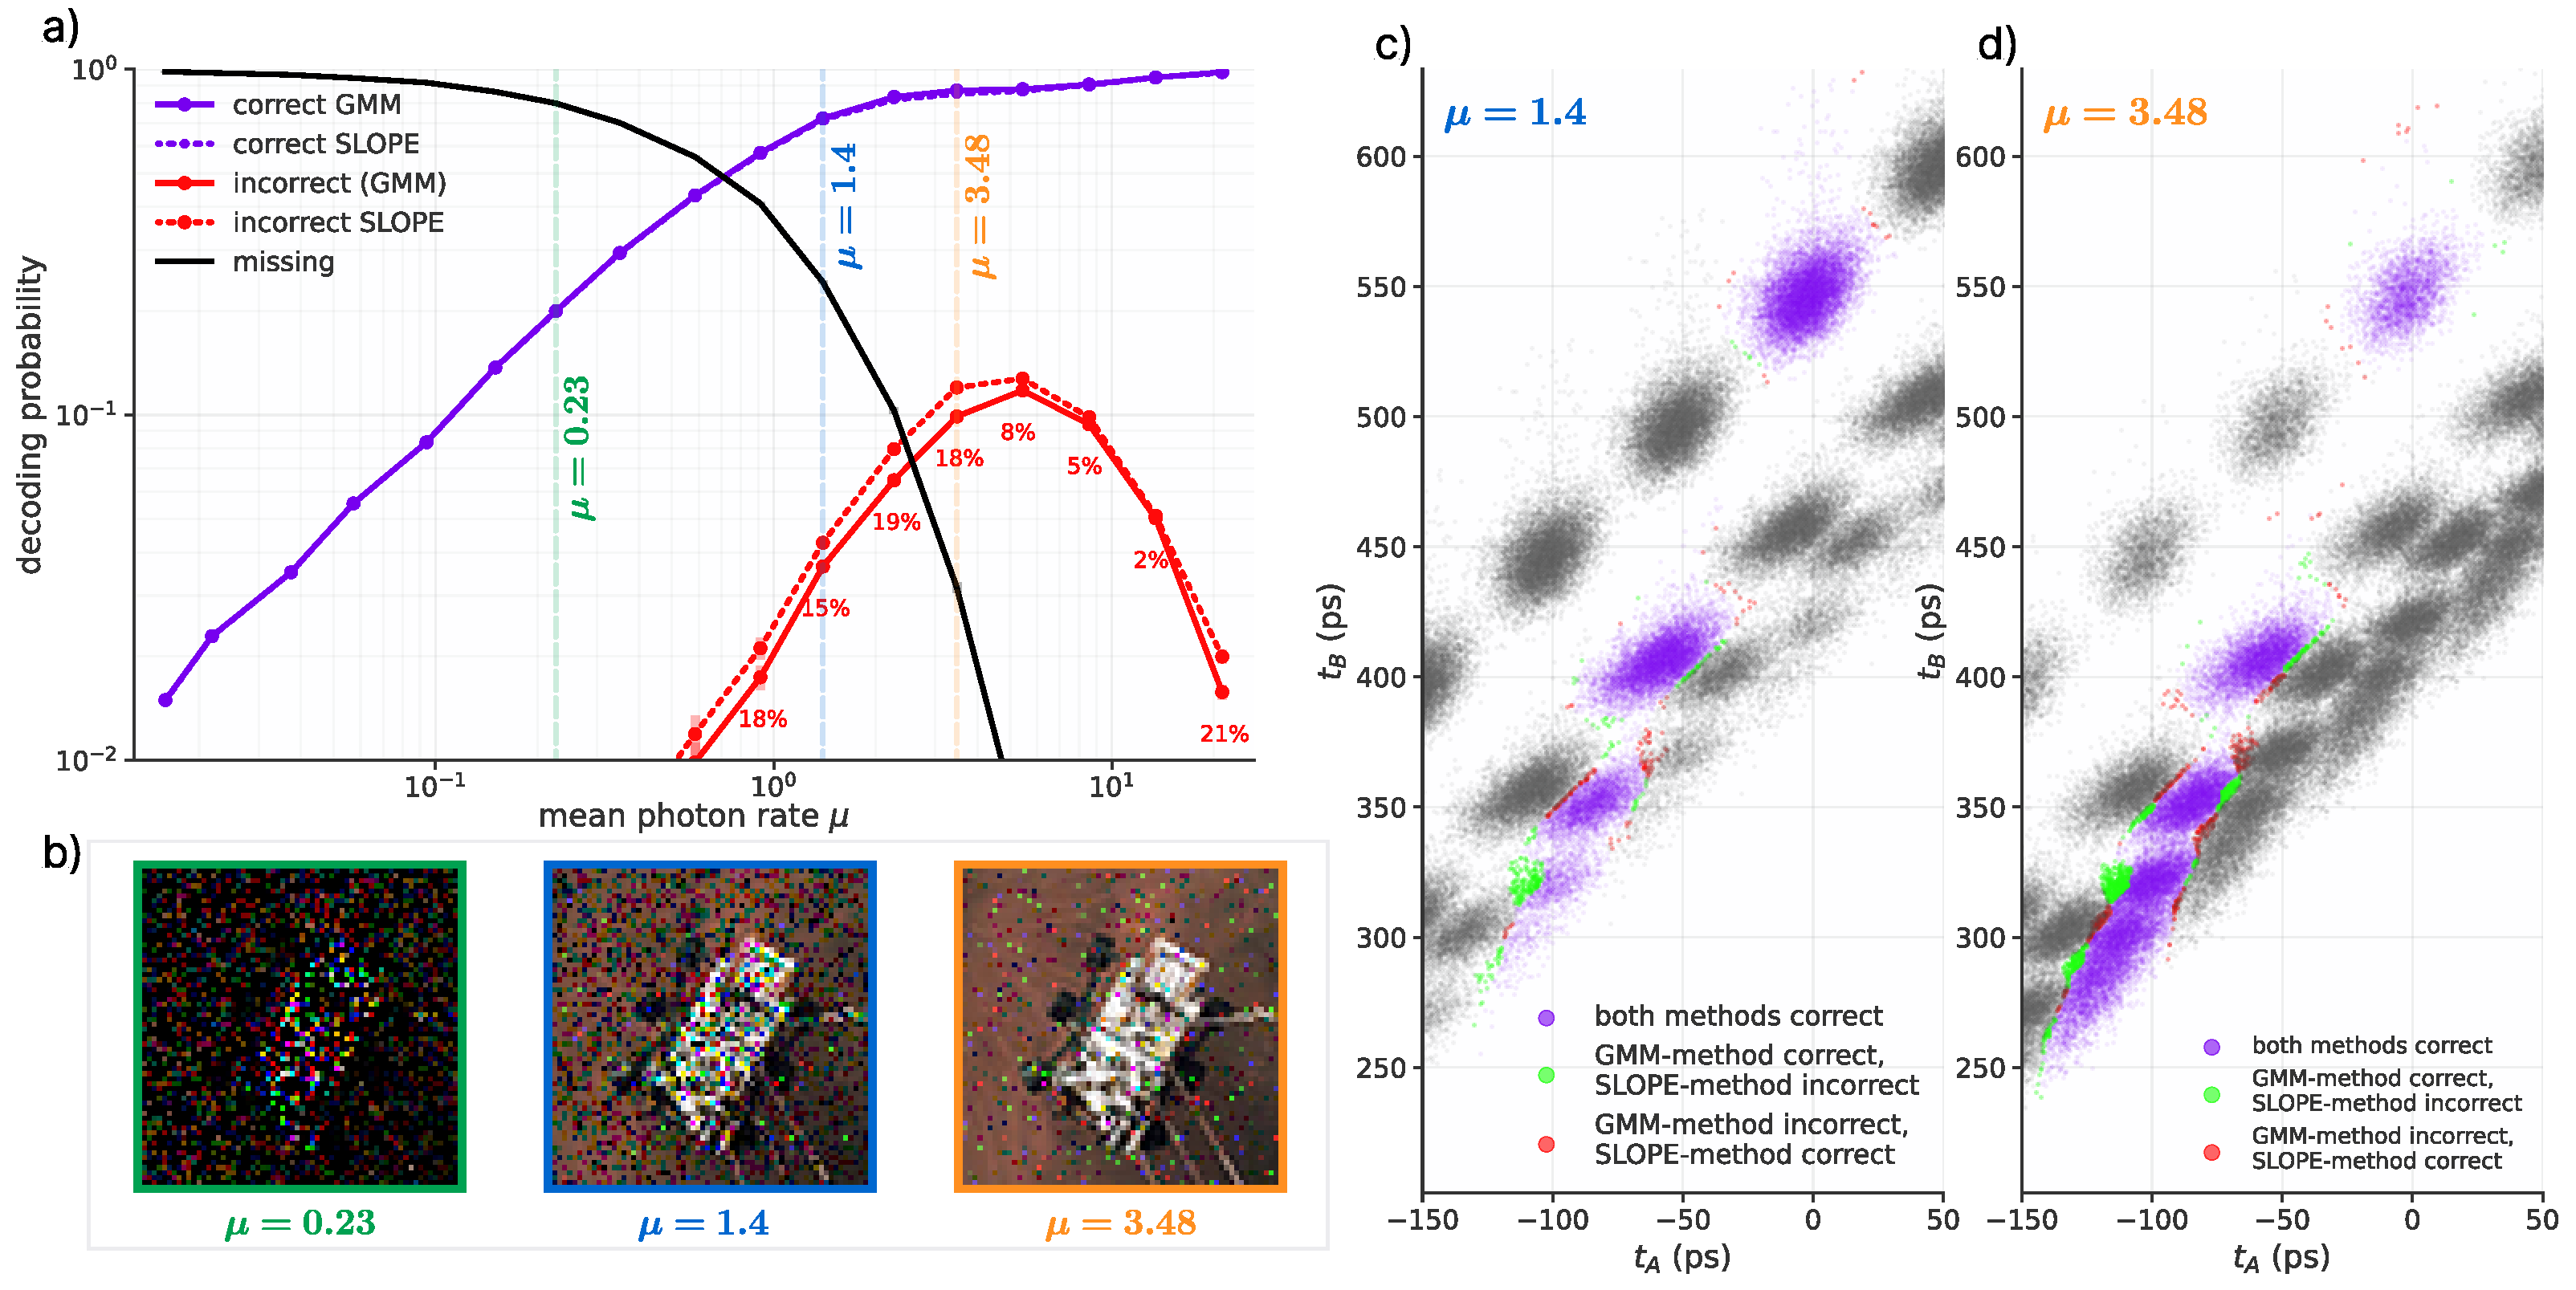
\includegraphics[width=1\textwidth]{./figs/ppm_decoding_20GHz_light.pdf}
\caption[{PPM decoding performance at 20~GHz}]{\textbf{PPM decoding performance at 20~GHz} a) ratios pulses making up the dataset that are missing, decoded correctly, or decoded incorrectly. The use of the GMM model reduces the the decoding error rate by 2 to 19% (red percentages) for the range of mean photon numbers for which the errors are most statistically significant as shown by the dashed red line. b) decoded images for three particular mean photon numbers, with the rate of correct bits specified in Mbits/s. Since no error correction is performed, these are just visual representations of the error rates shown above. c) \& d) Scatter plots showing the location of timing measurements $t_A, t_B$ from the PPM decoding. For each $t_A,t_B$ pair, the correct timing offset $i*50~ps$ is subtracted off to form the purple distribution. Grey distributions are copies of the purple data translated by $50~ps$, included to show how data from different time bins and photon clusters overlaps. Green (red) points highlight events that switched from incorrectly (correctly) decoded to correctly (incorrectly) decoded with application of the GMM method after the SLOPE method.}
\label{fig:decoding_20GHz}
\end{figure}
}

\hypertarget{photon-number-discrimination}{%
\section{Photon number discrimination}\label{photon-number-discrimination}}

The GMM used requires a specified number of Gaussians to fit the whole distributions with no constraints on the number of Gaussians assigned to certain clusters. Therefore, for photon number discrimination, a method for grouping the Gaussians into sets that describe specific photon number clusters is needed. We start with data from a moderate mean photon number which displays clusters for photon numbers from 1 to 5+. We specify a number of Gaussians to model this distribution in the range of 15 to 20, which ensures that each cluster is faithfully modelled by the sum of a few Gaussians. We observe a minimal improvement the the model accuracy if more Gaussians are used.

Then, we compute the symmetric Kullback--Leibler (KL) divergence divergence between all pairs of Gaussians and represent this data in an adjacency matrix. The KL divergence is a measure of the similarity between two probability distributions, and may be computed from the respective means and covariance matrices of each Gaussian component.

The adjacency matrix can be thought of as a undirected graph where each node represents a Gaussian component and each edge represents the symmetric KL divergence between two Gaussians. We then use a community detection algorithm to group the Gaussians into sets that correspond to the photon number clusters. We use the Louvain method \cite{Blondel2008} for this purpose, implemented in the NetworkX python package.

fig.~\ref{fig:pnr_groupings} a shows the result of dividing the Gaussian components into groups $C_j$ that represent particular photon numbers $j$. As shown, this is done for a moderate mean photon number ($\mu=3.47$) for which all the clusters $|1\rangle$ through $|5+\rangle$ in the modelled dataset are present with non-negligible statistics. With this, the GMM model can be tuned to best represent the response of the detector at other mean photon numbers as well, by normalizing and scaling the relative amplitudes of each group $C_j$. fig.~\ref{fig:pnr_groupings} b a shows photon number attribution using this model. Each event from the PPM dataset is assigned a most probable photon number based on the GMM model and its location in the $t_A, t_B$ plane. As indicated by the black dashed ellipse, misattribution can occur bewteen $|2\rangle$ events in a time slot $t$ and $|3\rangle$ events in the next time slot $t+1$. This is because the $|2\rangle$ and $|3\rangle$ clusters overlap in the $t_A, t_B$ plane for the 20~GHz dataset. This is overlap is much less pronounced for the 10~GHz dataset. Such ambiguities fundamentally limit the minimum length time bin length needed for simultaneous photon arrival and photon number attribution. If the correct time-slot is known a priori and photon number attribution is only done for `correct' arrival time events, then the photon number assignment is more accurate as shown in fig.~\ref{fig:pnr_groupings} c.~

\hypertarget{fig:pnr_groupings}{%
\begin{figure}
\centering
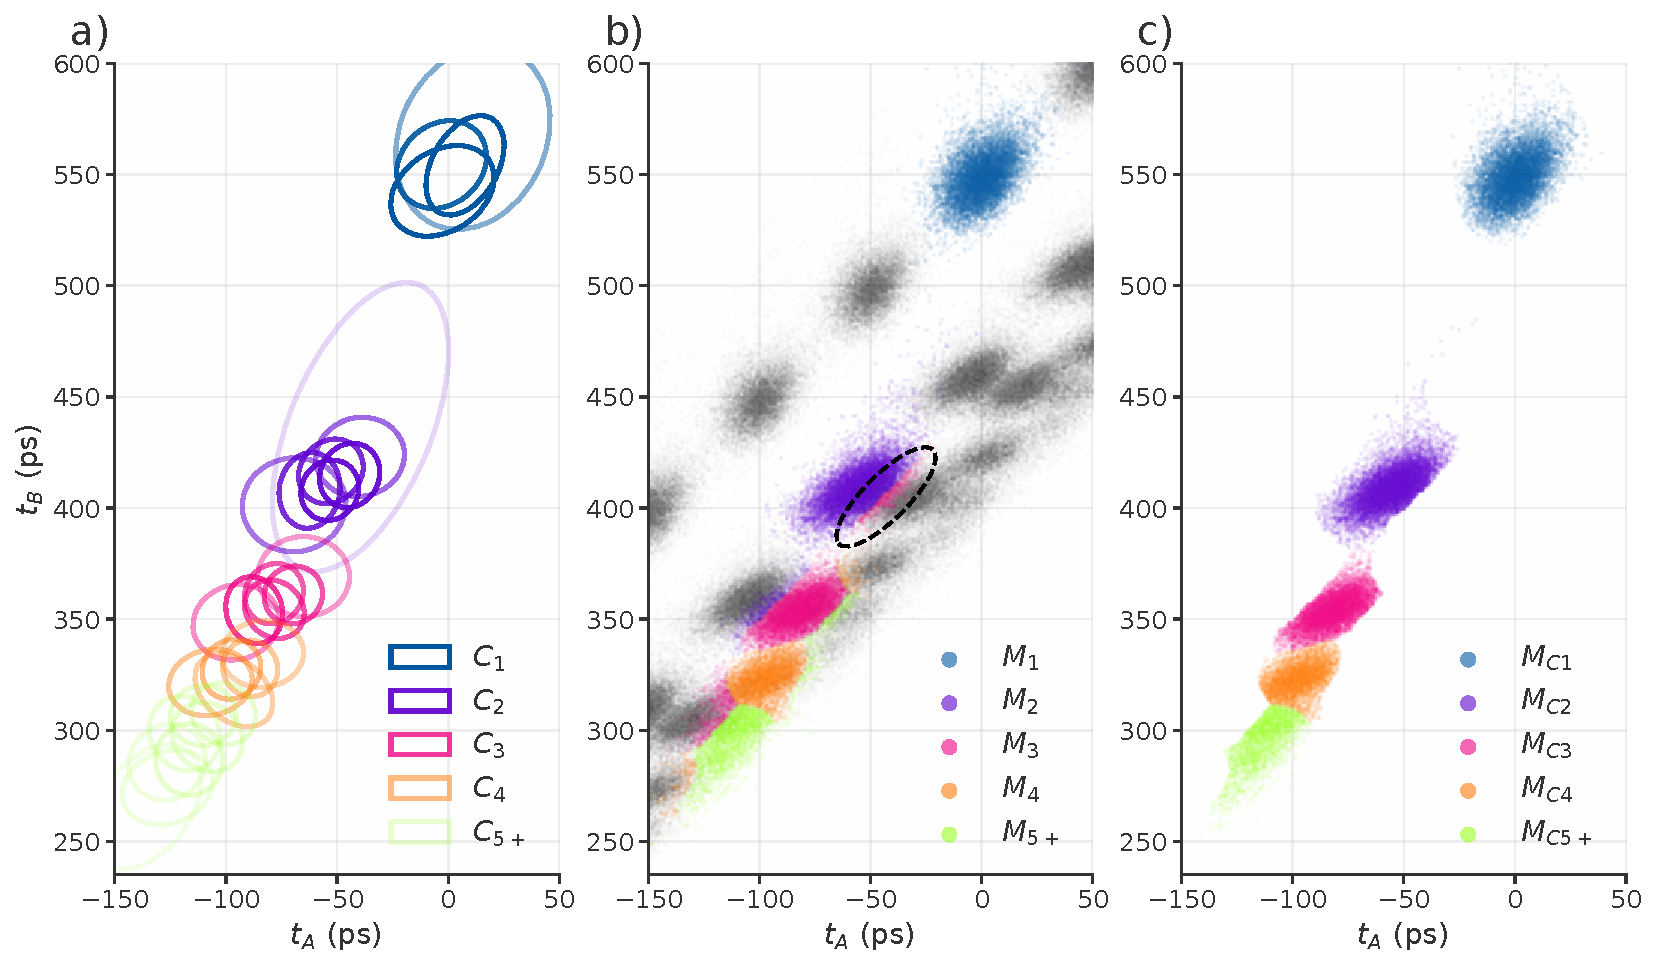
\includegraphics[width=1\textwidth]{./figs/pnr_resolved_arrival_time_groupings_light.pdf}
\caption[{Photon number attribution}]{\textbf{Photon number attribution} a) Ellipses represent Gaussians whose sum models the detector response for specific mean photon numbers. Ellipse opacity represents the Gaussian weight in the mixture. b) Photon number attribution with the 20~GHz dataset. Grey distributions are copies of the colored data for timeslot $i$ translated by $50~ps$ to show overlap c) Photon numbers assignments only for events that fall into the correct time bin.}
\label{fig:pnr_groupings}
\end{figure}
}

With measurements of photon number for each PPM event, the relative statistics of these events and vacuum events can be compared with the expected poisson statistics. fig.~\ref{fig:photon_statistics} shows the results of this comparison for the 20~GHz dataset. The measured statistics are in good agreement with the expected poisson statistics for the range of mean photon numbers tested.

\hypertarget{fig:photon_statistics}{%
\begin{figure}
\centering
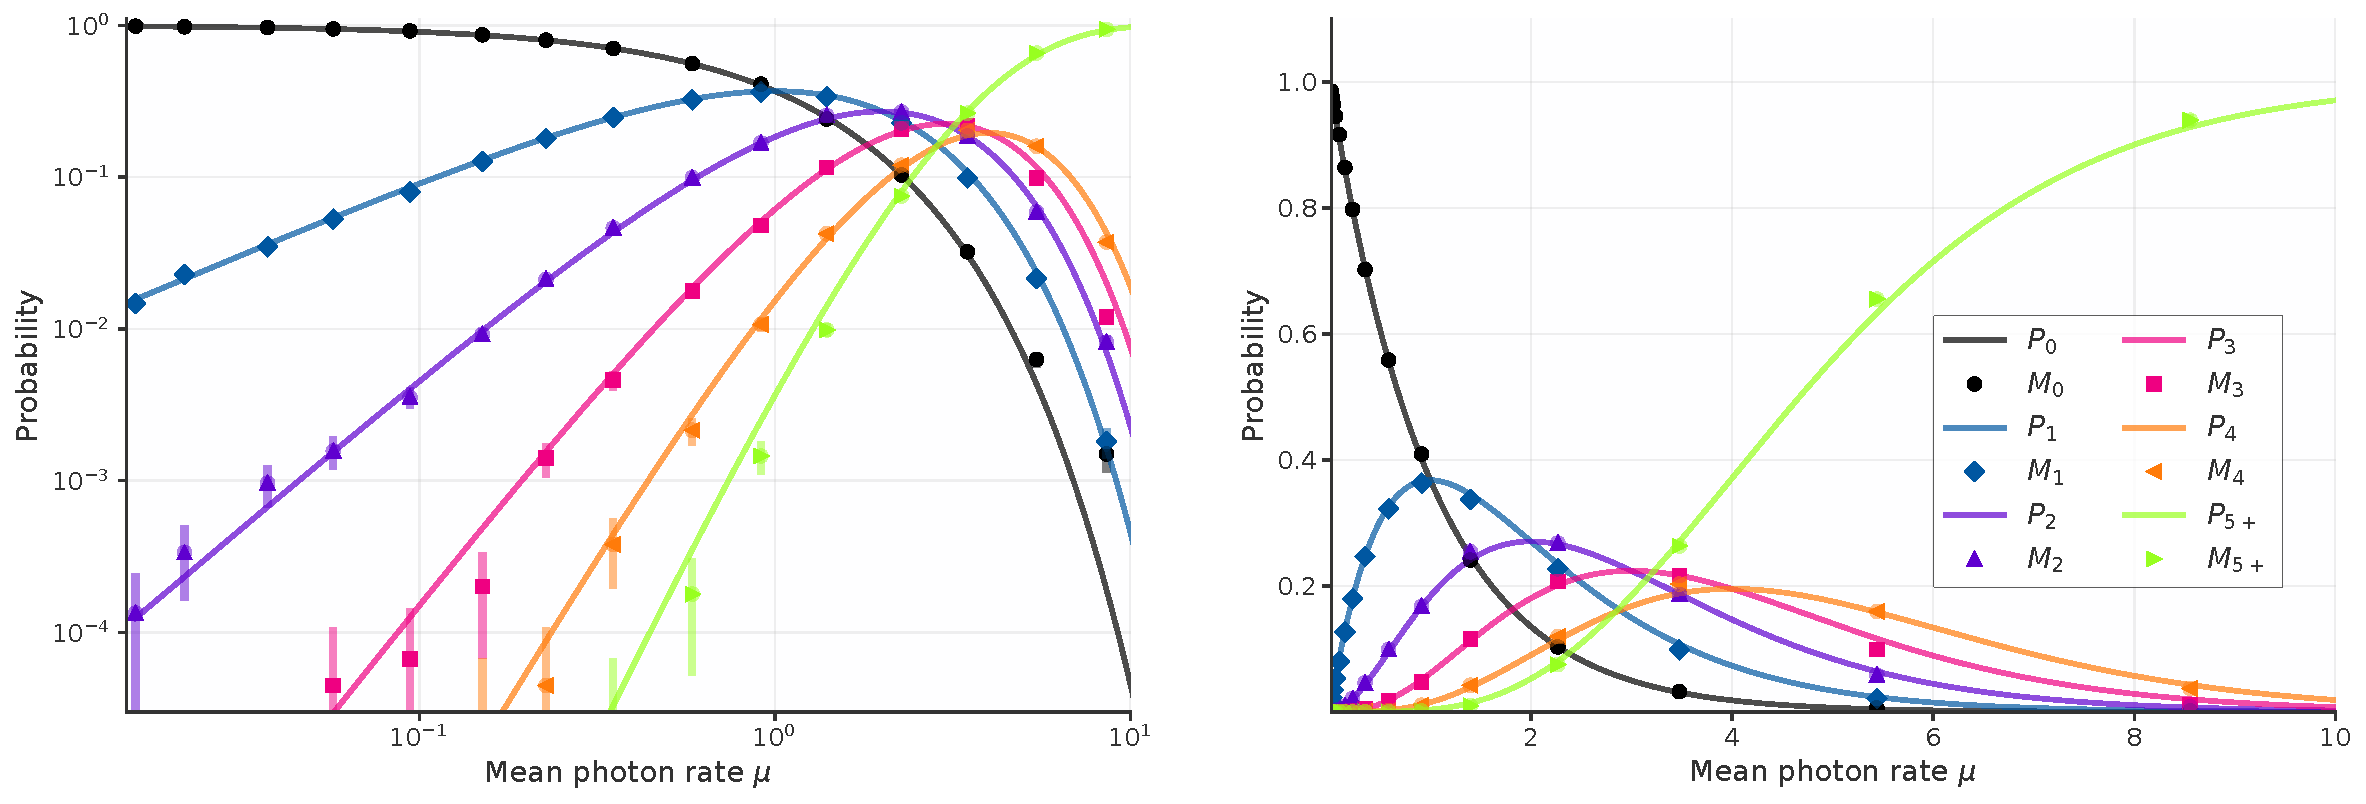
\includegraphics[width=1\textwidth]{./figs/pnr_stats_light.pdf}
\caption[{Photon number statistics}]{\textbf{Photon number statistics} Measured ( markers $M_j$ ) photon statistics overlayed with expected poisson statistics ( lines $P_j$ ) for the range of photon numbers tested. a) uses log-log scale, b) uses linear scale.}
\label{fig:photon_statistics}
\end{figure}
}

\hypertarget{discussion}{%
\section{Discussion}\label{discussion}}

We have shown that measurement of the slew rate or slope of SNSPD RF pulses may be useful for both photon number and arrival time discrimination. This is a fairly practical method that limited assumptions about the underlying modulation pattern of the optical signal. We show it allows for the measurement of pulse position modulation signals based on 10 and 20 Ghz clocks for which each optical pulse contains anywhere from 1 to 5 or more photons.

We also present a 2-dimensional Gaussian mixture model of the SNSPD response to the two trigger levels in an effort to model the available data as accurately and faithfully as possible. This may be used for photon number and arrival time discrimination as well. Assigning SNSPD detection events to photon number or PPM bins generalizes to assigning points in a 2-dimensional space to probability distributions built from Gaussian mixtures. We show the Gaussian mixture method moderately improves the accuracy of arrival time discrimination relative to the slope-based method.

The full 2D treatment of photon number discrimination based on community detection of Gaussian mixture groups is undeniably more complex than principle component analysis methods demonstrated in previous research \cite{sauer2023resolving, schapeler2023superconducting}. However, its generality may be advantageous for future SNSPD systems that gather added data about the transient state of the SNSPD and readout circuitry. For example, more than two timing measurements from each SNSPD pulse may prove to be useful. Recent research has demonstrated that photon number information is present in the falling edge of the pulse \cite{sauer2023resolving, schapeler2023superconducting}, and, as shown here, timing measurements from two trigger levels on the rising edge are useful. Therefore, the use of three or more unique time-correlated measurements may be advantageous. Digitizing the RF pulse with a high speed ADC or oscilloscope extends this thinking to many more measurements. Ultimately, photon number discrimination becomes a higher dimensional problem, for which Gaussian mixture methods may outperform principle component analysis.

Finally, higher dimensional analysis may be necessary when pulse overlap or time walk effects \cite{Mueller2023} complicate the nuanced photon number response characteristics of each SNSPD pulse. This is important in future SNSPD systems that are designed to exhibit both high maximum count rates \cite{Craiciu23} and photon number resolution.

\hypertarget{detector-figure-of-merit}{%
\section{Detector Figure of Merit}\label{detector-figure-of-merit}}

The work here highlights the application of low jitter single-photon detectors for optical communication, which is impactful for deep-space optical communication as well as classical communication in quantum networks. Although single-photon counting is well estanblished for deep-space optical communication~\cite{Srinivasan2023GroundReceiver} so far it has not been utilized in quantum networks, which have so far relied on off-the-shelf SFP modules and DWDMs. However, when quantum channels are frequency multiplexed with much higher power classical channels, Raman scattered photons from the classical channel pollute the quantum channel~\cite{EraerdsRaman}.

Attenuating classical communication to near the single photon level would solve this issue and require minimal added resources, as single photon detectors are already required at quantum nodes. DSOC demonstrates a promising approach to low-power classical communication based on phon counting and PPM which can be adapted for terrestrial quantum networks.

To access the applicability of different detectors, here we compare some of the recent near infrared detectors.

A useful figure of merit that includes all of the revelant detector metrics for photon timing was introduced by Bronzi and co-authors \cite{Bronzi2016}

$$FoM_T = \frac{\eta  (1 - P_{ap})\Phi_{-3 \text{dB}}}{J} \sqrt{\frac{A}{D}},$$

where $\eta$ is the single photon detection efficiency, $\Phi_{-3 \text{dB}}$ is the photon flux at which the system detection efficiency drops by 3~dB, $P_{ap}$ is the afterpulsing probability, $J$ is the detector jitter evaluated as the FWHM, $T_d$ is the deadtime, $A$ is the active area and $D$ is the dark count rate. Here we have defined the maximum photon flux as the 3~dB point, for ease of standardization.

In this work:

\begin{itemize}
\tightlist
\item
  Efficiency = 0.84
\item
  Afterpulsing = 0 %
\item
  Jitter = 15 ps
\item
  Deadtime = 30 ns \textbf{\hl{measure 3dB flux}}
\item
  Area = 330 $\mu m^2$
\item
  Dark count rate = 20~Hz
\end{itemize}

$FoM_T = 7.58 \times 10^{12}$ at 1550 nm.

The deadtime is calculated as the 1/MCR, which is the 3 dB point of the nominal efficiency. This is only a factor of 3.7 less than the state of the art visible Silicon SPADs (peak efficiency at 480~nm) \cite{Gramuglia2022}

In the future, the performance of the optical communication system could be improved by using high count rate SNSPD arrays. Recently published high-count rate arrays have figures of merit of \textbf{\hl{$FoM_T$ for Peacoq and Resta2023 results}}. This would result in a proportinal increase in the data rate.
\textbf{\hl{$FoM_T$ for fastest InGaAs/InP gated detector}}
These devices are ideal for fiber-based optical communication. In free-space, the active area is especially important, whithout the use of an adaptive optics system.
\textbf{\hl{$FoM_T$ for DSOC array}}

\bibliography{references}



\end{document}